
\de{ĐỀ THI HỌC KỲ I NĂM HỌC 2022-2023}{SGD Bắc Giang}


\begin{center}
	\textbf{PHẦN 1 - TRẮC NGHIỆM}
\end{center}
\Opensolutionfile{ans}[ans/ans]
\Opensolutionfile{ans}[ans/ans]
\begin{ex}%[0X2B3-3]%[Dự án đề HKI-HKII K10 NH22-23 (Cả nước), Nhật Thiện]%[Sở Bắc Giang]
	Cho khai triển $(7-8x)^5=a_0+a_1x+a_2x^2+a_3x^3+a_4x^4+a_5x^5$. Tính giá trị của biểu thức $S=a_0+a_1+a_2+a_3+a_4+a_5$.
	\choice
	{\True $S=-1$}
	{$S=0$}
	{$S=2$}
	{$S=1$}
\loigiai{
Ta có 
\begin{eqnarray*}
	(7-8x)^5&=& \mathrm{C}_5^5 7^5 (-8x)^0+\mathrm{C}_5^4 7^4 (-8x)^1+\mathrm{C}_5^3 7^3 (-8x)^2+\mathrm{C}_5^2 7^2 (-8x)^3+\mathrm{C}_5^1 7^1 (-8x)^4+\mathrm{C}_5^0 7^0 (-8x)^5\\
	&=&16807 - 96040 x + 219520 x^2 - 250880 x^3 + 143360 x^4 - 32768 x^5.
\end{eqnarray*}
Vậy biểu thức $S=16807 - 96040 + 219520 - 250880 + 143360 - 32768 =-1$.
}
\end{ex}
\begin{ex}%[0X1B3-2]%[Dự án đề HKI-HKII K10 NH22-23 (Cả nước), Nhật Thiện]%[Sở Bắc Giang]
	Khi kiểm tra ngẫu nhiên một số công nhân trong xí nghiệp, người ta thống kê lại độ tuổi của họ ở bảng sau
	\begin{center}
		\begin{tabular}{|c|c|c|c|c|c|c|}
			\hline
			Tuổi & $25$ & $26$ & $27$ & $29$ & $31$ & $34$\\
			\hline
			Số công nhân & $4$ & $9$ & $8$ & $3$ & $1$ & $1$\\
			\hline
		\end{tabular}
	\end{center}
Tìm trung vị của mẫu số liệu trên.
\choice
{$27$}
{$26$}
{$25{,}6$}
{\True $26{,}5$}
\loigiai{
Sắp xếp mẫu số liệu theo thứ tự không giảm
\begin{center}
	\begin{tabular}{|c|c|c|c|c|c|c|}
		$25$ & $25$ & $25$ & $25$ & $26$ & $26$ & $26$ \\
		$26$ & $26$ & $26$ & $26$ & $26$ & $26$ & $27$\\
		$27$ & $27$ & $27$ & $27$ & $27$ & $27$ & $27$\\
		& $29$ & $29$ & $29$ & $31$ & $34$ & \\
	\end{tabular}
\end{center}
Mẫu số liệu trên có $26$ giá trị. \\
Số hạng thứ mười ba và mười bốn lần lượt là $26$ và $27$.\\
Trung vị của mẫu số liệu trên là $M=\dfrac{26+27}{2}=26{,}5$.
}
\end{ex}
\begin{ex}%[0H3B1-3]%[Dự án đề HKI-HKII K10 NH22-23 (Cả nước), Nhật Thiện]%[Sở Bắc Giang]
	Trong mặt phẳng tọa độ $Oxy$, cho hai điểm $A(-3;1)$ và $B(6;5)$. Tìm tọa độ trọng tâm $G$ của tam giác $OAB$ (với $O$ là gốc tọa độ).
	\choice
	{$G\left(\dfrac{3}{2};3\right)$}
	{$G\left(3;\dfrac{4}{3}\right)$}
	{\True $G(1;2)$}
	{$G(2;1)$}
\loigiai{
Tọa độ trọng tâm $G$ của tam giác $OAB$ thỏa
$$\heva{&x_G=\dfrac{x_A+x_B+x_O}{3}=1\\&y_G=\dfrac{y_A+y_B+y_O}{3}=2.}$$
Vậy $G(1;2)$.
}
\end{ex}
\begin{ex}%[0X2B2-5]%[Dự án đề HKI-HKII K10 NH22-23 (Cả nước), Nhật Thiện]%[Sở Bắc Giang]
	Từ các chữ số $0$, $1$, $2$, $3$, $4$, $5$ có thể lập được bao nhiêu số tự nhiên chẵn và có $4$ chữ số khác nhau?
	\choice
	{$752$}
	{\True $156$}
	{$240$}
	{$160$}
\loigiai{
Gọi $\overline{abcd}$ là số tự nhiên chẵn có $4$ chữ số khác nhau.
Xét trường hợp $d=0$, ta có $1$ cách chọn.\\
Khi đó chọn $a$, $b$, $c$ có $\mathrm{A}_5^3$ cách chọn.\\
Suy ra trường hợp này có $1\cdot \mathrm{A}_5^3=180$.
Xét trường hợp $d$ là số chẵn khác $0$, ta có $2$ cách chọn.\\
Chọn $a\ne 0$ có $4$ cách. Khi đó chọn $b$, $c$ có $\mathrm{A}_4^2$ cách chọn.\\
Suy ra trường hợp này có $2\cdot 4\mathrm{A}_4^2=96$.\\
Vậy theo quy tắc cộng, có $60+96=156$ số thỏa mãn bài toán.
}
\end{ex}
\begin{ex}%[0X2B2-4]%[Dự án đề HKI-HKII K10 NH22-23 (Cả nước), Nhật Thiện]%[Sở Bắc Giang]
	Trong mặt phẳng cho $12$ điểm phân biệt trong đó không có $3$ điểm nào thẳng hàng. Số tam giác có $3$ đỉnh là $3$ trong $12$ điểm đã cho là
	\choice
	{$12^3$}
	{\True $\mathrm{C}_{12}^3$}
	{$12!$}
	{$\mathrm{A}_{12}^3$}
\loigiai{
Số tam giác được tạo ra là một tổ hợp chập $3$ của $12$ phần tử.
}
\end{ex}
\begin{ex}%[0X2K2-5]%[Dự án đề HKI-HKII K10 NH22-23 (Cả nước), Nhật Thiện]%[Sở Bắc Giang]
	Từ các chữ số $1$, $2$, $3$, $4$, $5$, $6$, $7$, $8$, $9$ có thể lập được bao nhiêu số tự nhiên có $4$ chữ số đôi một khác nhau và không có hai chữ số liên tiếp nào cùng chẵn?
	\choice
	{$960$}
	{\True $1800$}
	{$1680$}
	{$840$}
\loigiai{
	Gọi số cần tìm là $\overline{abcd}$.
	\begin{description}
		\item[Trường hợp 1:] Số cần tìm có $2$ chữ số chẵn, $2$ chữ số lẻ.\\
		Chọn $2$ số lẻ và xếp chúng vào $2$ chỗ có $\mathrm{A}_5^2$ cách.\\
		Chọn $2$ số chẵn và xếp vào $3$ khe trống tạo ra giữa $2$ số lẻ có $\mathrm{C}_4^2\cdot \mathrm{A}_3^2$ cách.\\
		Trường hợp này có $\mathrm{A}_5^2\cdot \mathrm{C}_4^2\cdot \mathrm{A}_3^2=720$ số.
		\item[Trường hợp 2:] Số cần tìm có $1$ chữ số chẵn, $3$ chữ số lẻ.\\
		Chọn $1$ chữ số chẵn và $3$ chữ số lẻ có $\mathrm{C}_4^1\cdot \mathrm{C}_5^3$ cách.\\
		Hoán vị $4$ chữ số này có $4!$ cách.
		Trường hợp này có $\mathrm{C}_4^1\cdot \mathrm{C}_5^3\cdot 4!=960$ số.
		\item[Trường hợp 3:] Số cần tìm có $4$ chữ số lẻ.\\
		Trường hợp này có $\mathrm{A}_5^4=120$ số.\\
	\end{description}
	Theo quy tắc cộng, có $720+960+120=1800$ số thỏa mãn.
}
\end{ex}
\begin{ex}%[0X2B2-5]%[Dự án đề HKI-HKII K10 NH22-23 (Cả nước), Nhật Thiện]%[Sở Bắc Giang]
	Từ các chữ số $1$, $2$, $3$, $4$ có thể lập được bao nhiêu số tự nhiên có $4$ chữ số đôi một khác nhau?
	\choice
	{$42$}
	{$265$}
	{\True $24$}
	{$256$}
\loigiai{
Từ các chữ số $1$, $2$, $3$, $4$ có thể lập được $4!=24$ số có $4$ chữ số đôi một khác nhau.
}
\end{ex}
\begin{ex}%[0X2K3-2]%[Dự án đề HKI-HKII K10 NH22-23 (Cả nước), Nhật Thiện]%[Sở Bắc Giang]
	Tìm hệ số của $x^3$ trong khai triển $f(x)=(1+x)^3+(1+x)^4+(1+x)^5$ thành đa thức.
	\choice
	{$16$}
	{$10$}
	{\True $15$}
	{$14$}
\loigiai{
Xét khai triển $(1+x)^3=1+3x+3x^2+x^3$.\\
Xét khai triển $(1+x)^4=1+4x+6x^2+4x^3+x^4$.\\
Xét khai triển $(1+x)^5=1+5x+10x^2+10x^3+5x^4+x^5$.\\
Vậy hệ số của $x^3$ trong khai triển $f(x)=(1+x)^3+(1+x)^4+(1+x)^5$ thành đa thức là
$1+4+10=15$.
}
\end{ex}
\begin{ex}%[0X2B2-4]%[Dự án đề HKI-HKII K10 NH22-23 (Cả nước), Nhật Thiện]%[Sở Bắc Giang]
	Trên mặt phẳng cho lục giác $ABCDEF$. Hỏi có bao nhiêu véc-tơ khác véc-tơ $\overrightarrow{0}$ và có điểm đầu, điểm cuối là $2$ trong $6$ đỉnh của lục giác đã cho?
	\choice
	{$36$}
	{\True $30$}
	{$11$}
	{$25$}
\loigiai{
Chọn $2$ trong $6$ đỉnh và hoán vị chúng, ta được $\mathrm{A}_6^2=30$ véc-tơ khác véc-tơ $\overrightarrow{0}$.
}
\end{ex}
\begin{ex}%[0X2B3-1]%[Dự án đề HKI-HKII K10 NH22-23 (Cả nước), Nhật Thiện]%[Sở Bắc Giang]
	Khai triển $(3x-5)^5$ thành đa thức có tất cả bao nhiêu số hạng?
	\choice
	{$5$}
	{$4$}
	{$7$}
	{\True $6$}
\loigiai{
Khai triển $(3x-5)^5$ thành đa thức với $n=5$ nên có $6$ số hạng.
}
\end{ex}
\begin{ex}%[0H4B2-3]%[Dự án đề HKI-HKII K10 NH22-23 (Cả nước), Nhật Thiện]%[Sở Bắc Giang]
	Trong mặt phẳng tọa độ $Oxy$, cho đường tròn $(C)\colon x^2+y^2+2x-6y+5=0$. Gọi $\Delta$ là tiếp tuyến của $(C)$ tại điểm $A(0;1)$. Phương trình tổng quát của $\Delta$ là
	\choice
	{$x-2y+1=0$}
	{$x+2y-2=0$}
	{$x+2y+2=0$}
	{\True $x-2y+2=0$}
\loigiai{
Đường tròn $(C)$ có tâm $I(-1;3)$.\\
Phương trình tiếp tuyến $\Delta$ của $(C)$ tại $A(0;1)$ nhận véc-tơ $\overrightarrow{IA}=(1;-2)$ làm véc-tơ pháp tuyến có dạng
$$\Delta\colon 1(x-0)-2(y-1)=0\Leftrightarrow x-2y+2=0.$$
}
\end{ex}
\begin{ex}%[0X1B1-3]%[Dự án đề HKI-HKII K10 NH22-23 (Cả nước), Nhật Thiện]%[Sở Bắc Giang]
	Số quy tròn của số $5{,}1472$ với độ chính xác $d=0{,}05$ là
	\choice
	{$5$}
	{$5{,}15$}
	{\True $5{,}1$}
	{$5{,}2$}
\loigiai{
Số quy tròn của số $5{,}1472$ với độ chính xác $d=0{,}05$ là $5{,}1$.
}
\end{ex}
\begin{ex}%[0H4B2-1]%[Dự án đề HKI-HKII K10 NH22-23 (Cả nước), Nhật Thiện]%[Sở Bắc Giang]
	Trong mặt phẳng tọa độ $Oxy$, cho đường tròn $(C)\colon (x-1)^2+(y+3)^2=16$. Tọa độ tâm $I$ của đường tròn $(C)$ là
	\choice
	{\True $(1;-3)$}
	{$(-3;1)$}
	{$(-1;-3)$}
	{$(1;3)$}
\loigiai{
Tọa độ tâm $I$ của đường tròn $(C)$ là $(1;-3)$
}
\end{ex}
\begin{ex}%[0X1B3-1]%[Dự án đề HKI-HKII K10 NH22-23 (Cả nước), Nhật Thiện]%[Sở Bắc Giang]
	Thống kê số cuốn sách mỗi bạn trong lớp đã đọc trong năm $2022$, Nga thu được kết quả như bảng bên dưới. Hỏi trong năm $2022$, trung bình mỗi bạn trong lớp của Nga đọc được bao nhiêu cuốn sách?
	\begin{center}
		\begin{tabular}{|c|c|c|c|c|c|}
			\hline
			Số cuốn sách & $1$ & $2$ & $3$ & $4$ & $5$\\
			\hline
			Số bạn & $3$ & $5$ & $15$ & $10$ & $7$\\
			\hline
		\end{tabular}
	\end{center}
\choice
{\True $3{,}325$}
{$2{,}325$}
{$4{,}325$}
{$3{,}5$}
\loigiai{
Trung bình của mẫu số liệu đã cho là
$$\overline{x}=\dfrac{1\cdot 3+2\cdot 5+3\cdot 15+4\cdot 10+5\cdot 7}{3+5+15+10+7}=3{,}325.$$\\
Vậy trung bình mỗi bạn trong lớp Nga đọc được $3{,}325$ cuốn sách.
}
\end{ex}
\begin{ex}%[0H4B1-5]%[Dự án đề HKI-HKII K10 NH22-23 (Cả nước), Nhật Thiện]%[Sở Bắc Giang]
	Trong mặt phẳng tọa độ $Oxy$, cho đường thẳng $d\colon 3x+4y+3=0$. Khoảng cách từ điểm $A(2;4)$ đến đường thẳng $d$ bằng
	\choice
	{\True $5$}
	{$\dfrac{4}{5}$}
	{$\dfrac{1}{5}$}
	{$4$}
\loigiai{
Khoảng cách từ điểm $A(2;4)$ đến đường thẳng $d$ bằng
$$\mathrm{d}(A,d)=\dfrac{|3\cdot 2+4\cdot 4+3|}{\sqrt{3^2+4^2}}=\dfrac{25}{5}=5.$$
}
\end{ex}
\begin{ex}%[0H3B1-2]%[Dự án đề HKI-HKII K10 NH22-23 (Cả nước), Nhật Thiện]%[Sở Bắc Giang]
	Trong mặt phẳng tọa độ $Oxy$, cho hai véc-tơ $\overrightarrow{a}=(2;-1)$ và $\overrightarrow{b}=(1;5)$. Tìm tọa độ của véc-tơ $\overrightarrow{a}-\overrightarrow{b}$.
	\choice
	{$(1;-4)$}
	{$(-1;6)$}
	{$(-1;-6)$}
	{\True $(1;-6)$}
\loigiai{
Ta có $\overrightarrow{a}-\overrightarrow{b}=(1;-6)$.
}
\end{ex}
\begin{ex}%[0X2B1-1]%[Dự án đề HKI-HKII K10 NH22-23 (Cả nước), Nhật Thiện]%[Sở Bắc Giang]
	Bạn An có $4$ quyển sách Toán học, $6$ quyển sách Văn học và $5$ quyển sách Tiếng Anh, các quyển sách là khác nhau. Hỏi bạn AN có bao nhiêu cách chọn một quyển sách để đọc?
	\choice
	{$120$}
	{$11$}
	{$10$}
	{\True $15$}
\loigiai{
Theo quy tắc cộng, An có $4+6+5=15$ cách chọn một quyển sách để đọc.
}
\end{ex}
\begin{ex}%[0H4B3-1]%[Dự án đề HKI-HKII K10 NH22-23 (Cả nước), Nhật Thiện]%[Sở Bắc Giang]
	Trong mặt phẳng tọa độ $Oxy$, cho Elip có phương trình chính tắc $\dfrac{x^2}{34}+\dfrac{y^2}{9}=1$. Điểm nào dưới đây là một tiêu điểm của Elip đã cho?
	\choice
	{$F_1(-3;0)$}
	{\True $F_2(-5;0)$}
	{$F_3(0;-5)$}
	{$F_4(\sqrt{34};0)$}
\loigiai{
Ta có $a^2=34$, $b^2=9$ suy ra $c^2=a^2-b^2=25$.\\
Vậy tiêu điểm của Elip đã cho lần lượt là $(-5;0)$ và $(5;0)$.
}
\end{ex}

\begin{ex}%[0X2B2-3]%[Dự án đề HKI-HKII K10 NH22-23 (Cả nước), Nhật Thiện]%[Sở Bắc Giang]
	Mật khẩu của một trang web là một dãy có từ $2$ tới $3$ kí tự, trong đó kí tự đầu tiên là một trong $26$ chữ cái in thường trong bảng chữ cái tiếng Anh (từ a đến z), mỗi kí tự còn lại là một chữ số từ $0$ đến $9$. Hỏi có thể tạo ra được bao nhiêu mật khẩu khác nhau?
	\choice
	{\True $2600$}
	{$260$}
	{$2860$}
	{$676$}
\loigiai{
Trường hợp mật khẩu của trang web là một dãy có $2$ kí tự.\\
Khi đó kí tự đầu có $26$ cách chọn, kí tự còn lại có $10$ cách chọn.\\
Suy ra trường hợp này có $26\cdot 10=260$ cách chọn.\\
Trường hợp mật khẩu của trang web là một dãy có $3$ kí tự.\\
Khi đó kí tự đầu có $26$ cách chọn, $2$ kí tự còn lại có $\mathrm{A}_{10}^2$ cách chọn.\\
Suy ra trường hợp này có $26\cdot \mathrm{A}_{10}^2=2340$ cách chọn.\\
Vậy có $2340+260=2600$ mật khẩu có thể được tạo ra.
}
\end{ex}
\begin{ex}%[0H4B1-1]%[Dự án đề HKI-HKII K10 NH22-23 (Cả nước), Nhật Thiện]%[Sở Bắc Giang]
	Trong mặt phẳng tọa độ $Oxy$, cho đường thẳng $d\colon 2x-3y+1=0$. Véc-tơ nào dưới đây là một véc-tơ pháp tuyến của đường thẳng $d$?
	\choice
	{\True $\overrightarrow{n}_1=(2;-3)$}
	{$\overrightarrow{n}_4=(3;2)$}
	{$\overrightarrow{n}_2=(2;3)$}
	{$\overrightarrow{n}_3=(3;-2)$}
\loigiai{
Đường thẳng $d\colon 2x-3y+1=0$ nhận $\overrightarrow{n}_1=(2;-3)$ làm một véc-tơ pháp tuyến.
}
\end{ex}


\Closesolutionfile{ans}
%\begin{center}
%	\textbf{ĐÁP ÁN}
%	\inputansbox{10}{ans/ans}	
%\end{center}
\begin{center}
	\textbf{PHẦN 2 - TỰ LUẬN}
\end{center}



%%%% Câu 1
\begin{bt}%[0H4Y1-1]%[0H4B1-2]%[Dự án đề kiểm tra HKII NH22-23 - Thành Đức Trung]%[Sở Bắc Giang]
Trong mặt phẳng tọa độ $Oxy$, cho hai điểm $A(2;2)$ và $B(4;-2)$.
\begin{enumerate}
\item Tìm tọa độ véc-tơ $\overrightarrow{AB}$.
\item Viết phương trình tổng quát của đường thẳng $AB$.
\end{enumerate}
\loigiai
{
\begin{enumerate}
\item Ta có $\overrightarrow{AB}=(2;-4)$.
\item Đường thẳng $AB$ nhận véc-tơ $\overrightarrow{AB}=(2;-4)$ làm véc-tơ chỉ phương.\\
Chọn véc-tơ pháp tuyến của đường thẳng $AB$ là $\overrightarrow{n}=(2;1)$.\\
Đường thẳng $AB$ đi qua điểm $A(2;2)$ nên phương trình tổng quát của đường thẳng $AB$ là
$$2(x-2)+1(y-2)=0 \Leftrightarrow 2x+y-6=0.$$
\end{enumerate}
}
\end{bt}

%%%% Câu 2
\begin{bt}%[0X2Y2-3]%[0X2B2-3]%[Dự án đề kiểm tra HKII NH22-23 - Thành Đức Trung]%[Sở Bắc Giang]
Một hộp chứa $5$ quả cầu trắng và $6$ quả cầu đỏ, các quả cầu có kích thước và khối lượng giống nhau.
\begin{enumerate}
\item Có bao nhiêu cách lấy ngẫu nhiên đồng thời $3$ quả cầu trong hộp?
\item Có bao nhiêu cách lấy ngẫu nhiên đồng thời $3$ quả cầu trong hộp sao cho trong $3$ quả cầu lấy ra có ít nhất một quả cầu trắng?
\end{enumerate}
\loigiai
{
\begin{enumerate}
\item Tổng số quả cầu trong hộp là $11$. \\
Vậy số cách lấy ngẫu nhiên đồng thời $3$ quả cầu trong hộp là
$$\mathrm{C}_{11}^3=165.$$
\item Số cách lấy ngẫu nhiên đồng thời $3$ quả cầu trong hộp sao cho $3$ quả cầu lấy ra có màu đỏ là
$$\mathrm{C}_{6}^{3}=20.$$
Vậy số cách lấy ngẫu nhiên đồng thời $3$ quả cầu trong hộp sao cho trong $3$ quả cầu lấy ra có ít nhất một quả cầu trắng là
$$165-20=145.$$
\end{enumerate}
}
\end{bt}

%%%% Câu 3
\begin{bt}%[0X2Y2-3]%[0X2B2-3]%[Dự án đề kiểm tra HKII NH22-23 - Thành Đức Trung]%[Sở Bắc Giang]
Tìm hệ số của $x^3$ trong khai triển $\left(3x-1\right)^5$.
\loigiai
{
Ta có
$$\begin{aligned}
\left(3x-1\right)^5
&=\mathrm{C}_5^0\cdot(3x)^5+\mathrm{C}_5^1\cdot(3x)^4\cdot(-1)+\cdots+\mathrm{C}_5^4\cdot(3x)^1\cdot(-1)^4+\mathrm{C}_5^5\cdot(-1)^5 \\
&=243x^5-405x^4+270x^3-90x^2+15x-1.
\end{aligned}$$
Vậy hệ số của $x^3$ trong khai triển $\left(3x-1\right)^5$ là $270$.
}
\end{bt}

%%%% Câu 4
\begin{bt}%[0H4K3-A]%[Dự án đề kiểm tra HKII NH22-23 - Thành Đức Trung]%[Sở Bắc Giang]
\immini{
Tháp giải nhiệt của một nhà máy có nóc và đáy là hai hình tròn, mặt cắt đứng của tháp được thiết kế có dạng hypebol (tham khảo hình vẽ). Biết khoảng cách giữa hai tiêu điểm của hypebol bằng $20$m, độ dài trục thực của hypebol bằng $16$m. Chiều cao của tháp bằng $125$m và khoảng cách từ nóc tháp đến tâm đối xứng của hypebol bằng $\dfrac{2}{3}$ khoảng cách từ tâm đối xứng đến đáy. Tính diện tích đáy của tháp.
}{
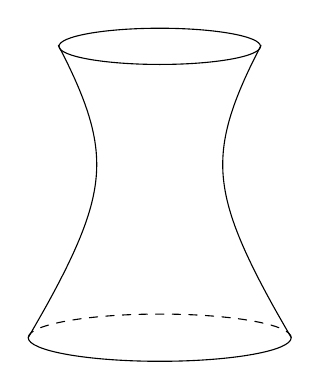
\begin{tikzpicture}[scale=2, font=\footnotesize, line join=round, line cap=round, >=stealth]
\draw[smooth, domain=-1.07:0.9]plot({0.4 / cos(\x r)}, {0.6 * tan(\x r)});
\draw[smooth, xscale=-1, domain=-1.07:0.9]plot({0.4 / cos(\x r)}, {0.6 * tan(\x r)});
\draw(-0.835,-1.1)arc(180:360:0.835cm and 0.15cm);
\draw[dashed](0.835,-1.1)arc(0:180:0.835cm and 0.15cm);
\draw(0.64,0.75)arc(0:360:0.64cm and 0.115cm);
\end{tikzpicture}
}
\loigiai{
\immini{
Chọn hệ trục tọa độ $Oxy$ như hình vẽ. \\
Phương trình chính tắc của hypebol có dạng $\dfrac{x^2}{a^2} - \dfrac{y^2}{b^2}=1$.\\
Theo giải thiết, ta có
\begin{itemize}
\item $F_1F_2 = 2c  =20\Rightarrow c=10$.
\item $A_1A_2 = 2a = 16\Rightarrow a=8$.
\end{itemize}
Suy ra $b = \sqrt{c^2 - a^2} = 6$. Do đó phương trình chính tắc của hypebol là
\[\dfrac{x^2}{64} - \dfrac{y^2}{36} =1.\qquad(*)\]
}{
\begin{tikzpicture}[scale=2, font=\footnotesize, line join=round, line cap=round, >=stealth]
\draw[-stealth] (-1.5,0)--(1.5,0)node[below]{$x$};
\draw[-stealth] (0,-1.5)--(0,1.5)node[left]{$y$};
\draw [smooth]  plot [domain=-1.1:1.1] ({0.4 / cos(\x r)}, {0.6 * tan(\x r)});
\draw [smooth,xscale=-1]  plot [domain=-1.1:1.1] ({0.4 / cos(\x r)}, {0.6 * tan(\x r)});
\fill (.8,0) node[above]{$F_2$} circle (.5pt);
\fill (-.8,0) node[above]{$F_1$} circle (.5pt);
\fill (-.4,0) node[above right]{$A_1$} circle (.5pt);
\fill (.4,0) node[above left]{$A_2$} circle (.5pt);
\fill (0,0) node[below right]{$O$} circle (.5pt);
\fill (-.835,-1.1) circle (.5pt);
\fill (.835,-1.1) circle (.5pt);
\fill (-.64,.75) circle (.5pt);
\fill (.64,.75) circle (.5pt);
\draw[thick] (-.835,-1.1)--(.835,-1.1) (-.64,.75)--(.64,.75);
\end{tikzpicture}
}
\noindent Gọi $z$ là khoảng cách từ tâm đối xứng của hypebol đến đáy tháp. Theo đề bài ta có phương trình
\[z + \dfrac{2}{3}z = 123\Leftrightarrow z=75.\]
Thay $y=  -75$ vào $(*)$ ta tìm được $x = \pm4\sqrt{629}$.\\
Suy ra bán kính đường tròn đáy là $R = 4\sqrt{629}$ mét. Khi đó diện tích đáy tháp là
\[S = \pi R^2 = 10064\pi \left(\text{m}^2\right).\]
}
\end{bt}